\documentclass[10pt]{article}
\usepackage[letterpaper,margin=0.55in]{geometry}
\usepackage[T1]{fontenc}
\usepackage{lmodern}
\usepackage{graphicx}
\usepackage{tabularx}
\usepackage{booktabs}
\usepackage{enumitem}
\usepackage{xcolor}
\usepackage{titlesec}
\usepackage{multicol}

\definecolor{navy}{HTML}{1F3A5F}
\definecolor{soft}{HTML}{EEF2F7}
\titleformat{\section}{\color{navy}\bfseries\normalsize}{}{0pt}{}
\titlespacing*{\section}{0pt}{5pt}{1pt}
\setlist{nosep,leftmargin=1.1em,topsep=1pt}
\setlength{\parindent}{0pt}
\setlength{\parskip}{3pt}
\setlength{\columnsep}{16pt}
\pagestyle{empty}

\begin{document}
\small

{\color{navy}\Large\bfseries Copart, Inc. (NASDAQ: CPRT)}\hfill{\color{navy}\bfseries\Large SHORT}\\[1pt]
{\footnotesize Price \$27.36 (Sep 30, 2026) \quad|\quad Price target \$21.50 ($-$21\%) \quad|\quad Market cap \$25.3B \quad|\quad 17.6x P/E \quad|\quad 11.1x EV/EBITDA \quad|\quad 6--12 mo.}

\vspace{3pt}
\colorbox{soft}{\parbox{\dimexpr\linewidth-2\fboxsep}{
\textbf{Recommendation: short CPRT, price target \$21.50 (21\% downside, 6--12 months).} Copart runs a toll road on wrecked cars and is paid per car, and fewer cars are using the road.\\[2pt]
\textbf{Thesis.} (1) \emph{Supply is shrinking for structural reasons:} drivers file fewer collision claims because insurance and repairs got expensive, and safer cars crash less. (2) \emph{Copart is losing share of what is left} to IAA, its only real rival. (3) \emph{Earnings are now falling:} fewer cars through fixed-cost yards cut profit faster than revenue, so the ``cheap'' multiple is a value trap.\\[2pt]
\textbf{Variant view.} The Street treats the 57\% drawdown as a cyclical dip to buy: the stock trades at 17.6x P/E vs.\ a 34x ten-year median, and consensus has FY27 EPS growing 11\% to \$1.75. We think the unit decline is structural and share-driven, so it will not reverse with the cycle. We see FY27 EPS of \$1.44, 18\% below the Street. Unlike every prior Copart drawdown, earnings are falling this time.}}

\section{Company overview}
Copart sells wrecked and unwanted vehicles through online auctions in the U.S. and abroad (19\% of Q4 FY26 revenue is international). When an insurer decides a car costs more to fix than it is worth (a total loss), it consigns the car to Copart, which tows, stores and sells it to rebuilders, dismantlers, exporters and dealers for buyer and seller fees. About 80\% of volume comes from insurers, so Copart's revenue depends on how many cars insurers total. FY26 (July year-end) revenue was \$4.67B (85\% service fees), operating income \$1.65B and EPS \$1.55. Copart holds \$4.5B of cash and securities with no meaningful debt, bought back \$1.6B of stock in FY26, and in September 2026 agreed to buy dealer wholesale marketplace ACV Auctions for $\sim$\$1.8B in cash.

\section{Industry: a two-player market fed by insurance claims}
U.S. salvage auctions are effectively a duopoly: Copart and IAA (owned by RB Global since 2023). Supply follows a simple chain: \emph{crash $\rightarrow$ claim $\rightarrow$ total loss $\rightarrow$ auction.} Rising repair costs push more claimed cars into total losses (a record 23.3\% of claims in Q2 2026, vs.\ 15.6\% in 2015), which lifts the value of each car. But Copart is paid per car, and the number of claims is falling. With total losses already near a quarter of claims, a higher total-loss rate can no longer make up for a shrinking base of claims.

\section{Thesis 1: The supply of wrecked cars is in structural decline}
\begin{itemize}
  \item \textbf{Expensive insurance and repairs push drivers out of the claims system (Exhibit 1C).} Since 2019, auto insurance prices are up 49\% and repair prices up 57\%, far ahead of 31\% overall inflation. Drivers respond by raising deductibles (26\% now carry \$1,000+), dropping collision cover and paying for small repairs themselves (7\% skipped a claim over rate worries, J.D. Power). Each of these is a crash that never becomes a claim, and so never becomes a Copart car. That is why collision claim frequency fell 3.4\% y/y in Copart's latest quarter and repairable claims fell 9.7\% in 2025 (CCC).
  \item \textbf{People are not driving less, so the problem is claims, not traffic (Exhibit 1C).} Miles driven are 2\% above 2019 and transit ridership is still 18\% below it, so as many cars are on the road as ever. Crash exposure has not fallen; claims have. This undercuts the bull case that volume returns as driving recovers: driving has already recovered and Copart's units still fell. Volume returns only if insurance gets cheap enough to bring drivers back to filing, and repair costs, still up 7.8\% y/y, push the other way.
  \item \textbf{Safer cars will shrink the pool for a decade.} Automatic emergency braking cuts rear-end crashes by $\sim$50\% (IIHS) and is mandatory on all new U.S. light vehicles from September 2029. As older cars are replaced, fewer crashes happen at all, which lowers Copart's supply even if claim filing recovers. This is a structural headwind, not a cycle to wait out.
\end{itemize}

\section{Thesis 2: Copart is losing share inside a shrinking market}
\begin{itemize}
  \item \textbf{IAA is winning the cars Copart loses (Exhibit 1A).} IAA's unit growth has beaten Copart's U.S. insurance units in every quarter since early 2025, by up to 18 points. If falling claims were the only problem, both companies would shrink together. Instead, over the last 12 months IAA grew 5.4\% while Copart fell 5.5\%, and the combined pool fell only 1.6\%. Most of Copart's decline is lost share, not a weak market.
  \item \textbf{The lost share is worth $\sim$\$166M of revenue a year (Exhibit 1B).} Copart's share of the two-player pool fell from 63.9\% to 61.4\% in one year, about 167k cars. At Copart's fee per car that is \$166M of service revenue, $\sim$4\% of the total, moving to a rival. It lands on yards whose costs do not fall with volume, so the hit to profit is larger than the hit to revenue (Thesis 3).
  \item \textbf{The lost customer is the insurer that is growing fastest.} Management said U.S. insurance units would have \emph{grown} 2.3\% in Q4 FY26 without one lost customer, vs.\ a 7.5\% decline reported. Industry reports name Progressive, now the largest U.S. auto insurer, which sends $\sim$90\% of its salvage to IAA. As Progressive adds policyholders, IAA adds cars automatically. IAA has also cut cycle times by nearly a week under RB Global, so Copart's old service edge over a poorly run rival is gone.
\end{itemize}

\section{Thesis 3: Falling earnings make the ``cheap'' multiple a trap}
\begin{itemize}
  \item \textbf{Fewer cars through fixed-cost yards means falling profit.} Copart pays for its yards, tow network and staff whether 4.0M or 4.5M cars arrive. In Q4 FY26 revenue per car rose 5.4\% but U.S. facility cost per car rose 14.2\%, so revenue grew 2.4\% while operating income fell 10.6\% and EPS fell 14.6\%. Higher car values no longer cover the cost of lost volume, and each further unit decline cuts profit faster than revenue.
  \item \textbf{The cash cushion under EPS is being spent.} Interest on Copart's cash (\$182M of other income) was about 10\% of FY26 net income. The ACV deal spends $\sim$\$1.8B of that cash, removing $\sim$\$0.06 of EPS before ACV's own losses, and management does not expect ACV to add to earnings until FY28. One support under EPS goes away just as the core business weakens.
  \item \textbf{Why buying the dip fails this time.} In Copart's five prior 30\%+ drawdowns, trailing EPS was still growing 10--46\%, so the stock recovered once sentiment turned. Today trailing EPS is down 3\% and falling, and a low P/E is only cheap if earnings hold. Since 1996, buying CPRT after weekly oversold signals returned a median $-$0.3\% over six months, vs.\ +9.9\% on a random day.
\end{itemize}

\vspace{2pt}
{\centering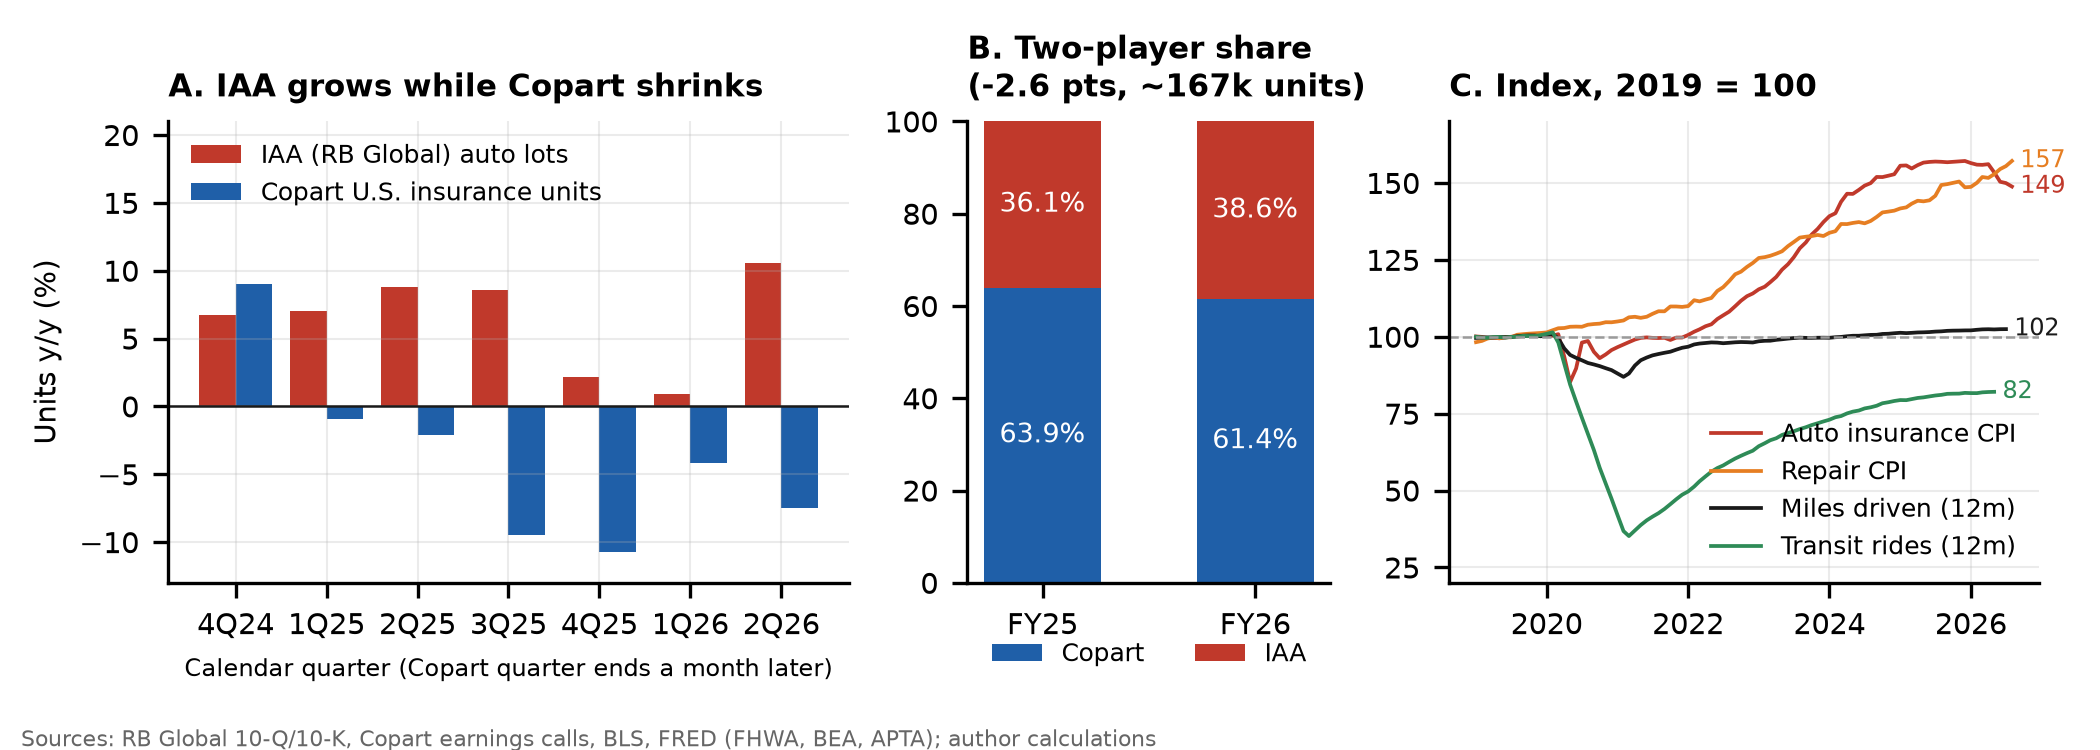
\includegraphics[width=0.84\linewidth]{../model/fundamentals/output/industry_figure.png}\par}
{\centering\footnotesize\textbf{Exhibit 1.} (A) Y/y unit growth: IAA has outgrown Copart's U.S. insurance units every quarter since early 2025. (B) Copart's share of the Copart + IAA pool fell 2.6 pts in a year. (C) 2019 = 100: insurance and repair prices are up 50\%+, pushing drivers to skip claims, while miles driven are flat and transit is down, so fewer claims does not mean less driving.\par}

\section{Valuation: FY27 EPS of \$1.44, 18\% below consensus}
We build FY27 EPS from units, revenue per unit and margin (Exhibit 2). In the base case, units fall 3\% as the lost insurer and falling claims carry into the first half, and revenue per unit rises 4\% on higher car values. Operating margin settles at 33\%, near the Q4 FY26 exit rate of 32\%, because fixed yard costs are spread over fewer cars, and other income falls to \$110M after the ACV payment. That gives \textbf{EPS of \$1.44 vs.\ the Street's \$1.75}. At 15x, a discount to share-gaining RB Global (16.8x forward) and a premium to salvage-parts buyer LKQ (7.4x), the base target is \textbf{\$21.50}. That implies 9.7x EV/EBITDA, below today's 11.1x.

\begin{center}
{\footnotesize\textbf{Exhibit 2.} FY27 EPS scenarios and price targets\\[2pt]
\begin{tabular}{@{}lrrrrrrrr@{}}
\toprule
Scenario (prob.) & Units & Rev./unit & Op. margin & FY27 EPS & vs.\ Street & P/E & Target & vs.\ price \\
\midrule
Bear (25\%) & $-$6\% & +3\% & 31.0\% & \$1.30 & $-$26\% & 13x & \$16.84 & $-$38\% \\
\textbf{Base (50\%)} & $\mathbf{-3\%}$ & \textbf{+4\%} & \textbf{33.0\%} & \textbf{\$1.44} & $\mathbf{-18\%}$ & \textbf{15x} & \textbf{\$21.54} & $\mathbf{-21\%}$ \\
Bull (25\%) & +2\% & +5\% & 36.5\% & \$1.70 & $-$3\% & 20x & \$33.90 & +24\% \\
\midrule
\multicolumn{7}{@{}l}{Probability-weighted} & \$23.45 & $-$14\% \\
\bottomrule
\end{tabular}}
\end{center}
\vspace{-4pt}
Probability-weighted, the expected downside ($\sim$20 pts) is more than 3x the expected upside ($\sim$6 pts), and even the bull case needs a unit recovery that no data point supports today.

\section{Catalysts}
\begin{itemize}
  \item \textbf{Q1 FY27 earnings (Nov 19, 2026).} Consensus is \$0.40 vs.\ \$0.41 a year ago. Another quarter of falling U.S. insurance units and cost-per-unit growth should push FY27 estimates toward our \$1.44.
  \item \textbf{RB Global Q3 results (early Nov 2026).} A seventh straight quarter of IAA unit gains would confirm the share shift is not a one-customer event.
  \item \textbf{ACV closing (by end of 2026).} Interest income falls and ACV's losses consolidate, pushing Copart into dealer wholesale, led by Manheim and OPENLANE, where it has no edge.
  \item \textbf{Monthly claims data.} Further declines in collision frequency and repairable claims (CCC, insurers) keep pressure on units.
\end{itemize}

\section{Risks and mitigants}
{\footnotesize
\begin{tabularx}{\linewidth}{@{}p{0.29\linewidth}X@{}}
\toprule
Risk & Mitigant \\
\midrule
Claims recover as insurance prices fall (auto insurance CPI $-$5.1\% y/y) & Repair prices are still rising (+7.8\% y/y) and deductibles are sticky, so small claims stay unfiled. AEB lowers crash frequency whatever insurance costs. We cover if collision frequency turns positive for two quarters. \\
Easier comps once the lost customer laps in early 2027 & The base case already assumes a smaller decline (units $-$3\%). The margin and interest-income pressure does not depend on the comp. \\
Hurricane season brings a burst of catastrophe volume & Catastrophe units are one-off and flatter revenue and units, not the trend. Copart reports volumes ex-catastrophe. \\
Buybacks and the ACV story support the stock & ACV uses $\sim$\$1.8B of the cash that funded buybacks. Short interest is only 4.6\% of float (3.3 days to cover), so squeeze risk is low. \\
Stock already down 57\% & Cheap on trailing P/E, but on our FY27 EPS the stock trades at 19x with falling units. We size the position with a stop at \$32.60 (above the 50-day average and the 23.6\% retracement). \\
\bottomrule
\end{tabularx}}

\vspace{2pt}
{\scriptsize\color{gray} Sources: Copart FY2026 10-K and Q4 FY26 earnings release and calls (FY25--FY26); RB Global 10-Q/10-K filings; CCC Intelligent Solutions Crash Course 2026; J.D. Power 2025 U.S. Auto Claims Satisfaction Study; IIHS; NHTSA FMVSS 127; BLS CPI; FRED (FHWA, APTA); Yahoo Finance prices and consensus (Sep 30, 2026); industry press on insurer allocations. Share estimates use Copart's stated $>$4M FY26 units; the share shift is $-$2.5 to $-$2.6 pts across a 4.0--4.5M unit range. Estimates and targets are the authors'.\par}
\end{document}
